\begin{figure}[htpb]
\centering
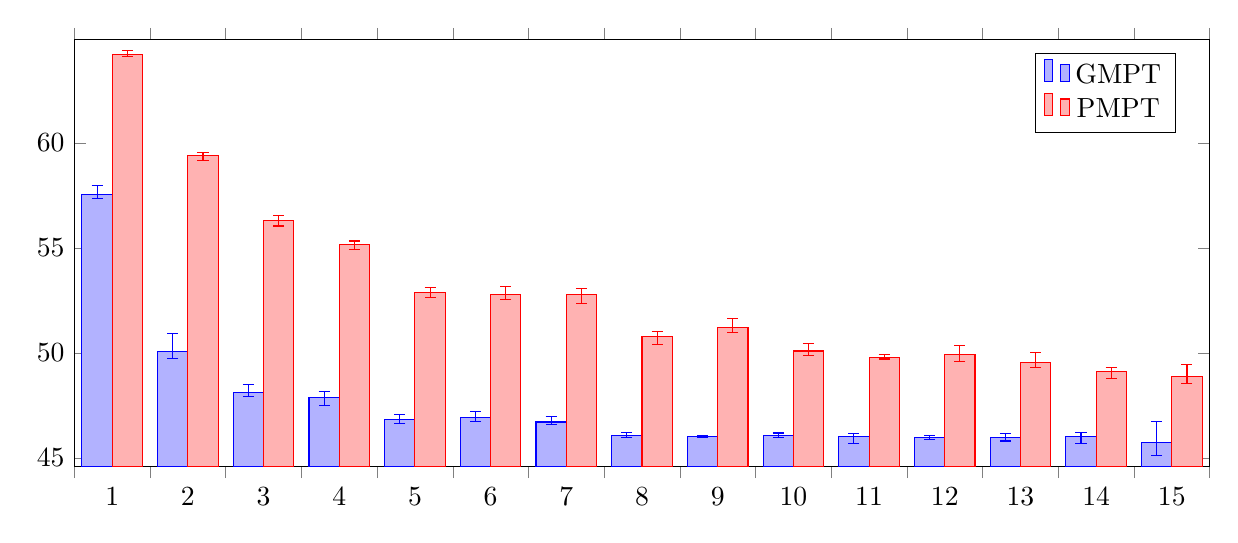
\begin{tikzpicture}
\begin{axis}[
legend pos=north east,
enlargelimits={abs=0.5},
ybar=0pt,
bar width=0.4,
width=16cm,
height=7cm,
xtick={0.5,1.5,...,15.5},
xticklabels={1,...,15},
x tick label as interval
]

\addplot+[error bars/.cd,
y dir=both,y explicit]
coordinates {
    (1,57.5520563450499) += (0,0.398853540814464) -= (0,0.201330990915480)
    (2,50.0604302920827) += (0,0.866091271257638) -= (0,0.331028154367644)
    (3,48.1349022236234) += (0,0.355946483631961) -= (0,0.222823054897276)
    (4,47.8792037719296) += (0,0.303108547127863) -= (0,0.363149943989576)
    (5,46.8457016899354) += (0,0.205369037718071) -= (0,0.189278375646438)
    (6,46.9471570620956) += (0,0.283919388811270) -= (0,0.190102634898516)
    (7,46.7123971085626) += (0,0.278914190099663) -= (0,0.125284290682778)
    (8,46.0886550528459) += (0,0.122945269276471) -= (0,0.111487151874172)
    (9,46.0242732290854) += (0,0.049294756670747) -= (0,0.038824599536404)
    (10,46.0722369733666) += (0,0.118787341594334) -= (0,0.097668077797919)
    (11,46.0081808167382) += (0,0.167245954957863) -= (0,0.330580162767291)
    (12,45.9802630984778) += (0,0.099632234016596) -= (0,0.109006019091346)
    (13,45.9581834222842) += (0,0.202949379069977) -= (0,0.146855052048636)
    (14,46.0288281215878) += (0,0.203512074431124) -= (0,0.337429725415305)
    (15,45.7433702432429) += (0,0.988790539494737) -= (0,0.642572318094373)};
\addplot+[error bars/.cd,
y dir=both,y explicit]
coordinates {
    (1,64.2241375751159) += (0,0.182334478026107) -= (0,0.105106255412579)
    (2,59.3849971691961) += (0,0.160117508425550) -= (0,0.210740141170646)
    (3,56.3173506236765) += (0,0.239900916080224) -= (0,0.274744049470343)
    (4,55.1580628740448) += (0,0.172019951671849) -= (0,0.225918485635077)
    (5,52.8662235798161) += (0,0.262029734087598) -= (0,0.232592431779267)
    (6,52.7709500297011) += (0,0.403868541815093) -= (0,0.244387502709799)
    (7,52.7962794542204) += (0,0.274615958449154) -= (0,0.432018339089105)
    (8,50.7854329474709) += (0,0.251981184023052) -= (0,0.379334349036014)
    (9,51.1949032354764) += (0,0.425712890855209) -= (0,0.215745383261044)
    (10,50.0938467841427) += (0,0.369880420433653) -= (0,0.193792365381015)
    (11,49.8023518920746) += (0,0.118029015092120) -= (0,0.088694652028841)
    (12,49.9302221875302) += (0,0.432539517210600) -= (0,0.355435124434486)
    (13,49.5657769865265) += (0,0.471659460816213) -= (0,0.253872889973046)
    (14,49.1236678371728) += (0,0.180139990117333) -= (0,0.339068851506454)
    (15,48.9006067806866) += (0,0.530949005299846) -= (0,0.342394440693489)};
\legend{GMPT,PMPT}
\end{axis}
\end{tikzpicture}
\caption[Comparison Multi-Task Notebook]{Comparison\footnotemark of the temperature measurements for GMPT and PMPT}
\label{fig:i_eva_gabar_n}
\end{figure}
\footnotetext{The bar values correspond to the median and the error bars correspond to the lower and upper inner fences displayed in the boxplots in \autoref{fig:i_eva_ga_n}}